\documentclass{../source/Experiment}

\major{信息工程}
\name{姚桂涛}
\title{基于FIR滤波器的离散预校正系统的设计和仿真验证}
\stuid{3190105597}
\college{信息与电子工程学院}
\date{\today}
\lab{}
\course{信号与系统}
\instructor{胡浩基}
\grades{}
\expname{离散预校正系统的设计和仿真验证}
\exptype{}
\partner{}
\begin{document}
    \makecover
    


    \section{问题的提出}
	数模转换器,又称D/A转换器,是把数字量转变成模拟量。在转换过程中,会产生较严重的频谱失真。
	
	而D/A转换器可以等效为一零阶保持电路,如果在其后面级联一个重建滤波器,在理想状态下,可以进行模拟信号的恢复。但是,该重建滤波器实际上很难实现。通过FIR滤波器,我们可以设计一个FIR滤波器与等效的零阶保持电路进行级联,从而实现预矫正,解决数模转换是频谱失真的问题。
	    
    \section{解决问题的原理、技术方案或算法}
        \subsection{数学模型}

            假设输入采样离散信号为$x[n]$,若直接通过一个零阶保持系统$H_o(j\omega)$进行恢复,
                
            $$H_o(j \omega)=T \frac{\sin (\omega T / 2)}{\omega T / 2}$$
            
            由于$H_o(j\omega)$并非一个理想的滤波器,其频谱图如下图所示,会产生信号频谱失真,而且$X(e^{j\omega})$越远离纵坐标轴时,失真越明显。
            
            为了解决其失真问题,可以在其零阶保持系统$Ho(j\omega)$加一个$Hr(j\omega)$,
            
            $$H r(j \omega)=\frac{1}{T} \frac{\omega T / 2}{\sin (\omega T / 2)},|\omega|<\omega_{c}$$
            
            使$H_o(j\omega)$与$Hr(j\omega)$级联后等效为一个理想滤波器,因此信号可得到精确恢复,转换过程如下图所示。

            \begin{figure}[H]
                \centering
                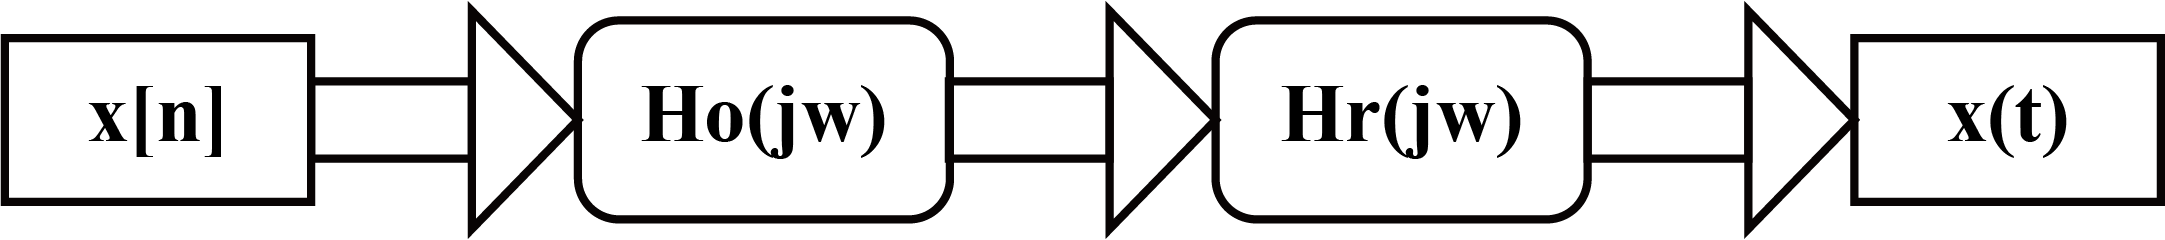
\includegraphics[width = 0.7\textwidth]{pic/sys1.png}
                \caption{连续预矫正系统}
            \end{figure}
            
            但是由于连续时间系统$Hr(j\omega)$是非因果系统,并且频率响应两边有上翘,在实际设计中几乎无法实现。所以可以将$Hr(j\omega)$提前作离散化处理,让信号先通过离散数字系统$Hr(e^{j\omega})$然后再通过零阶保持系统$Ho(j\omega)$,这样级联后的系统仍然等效为一个理想滤波器,转换过程如下图所示。

            \begin{figure}[H]
                \centering
                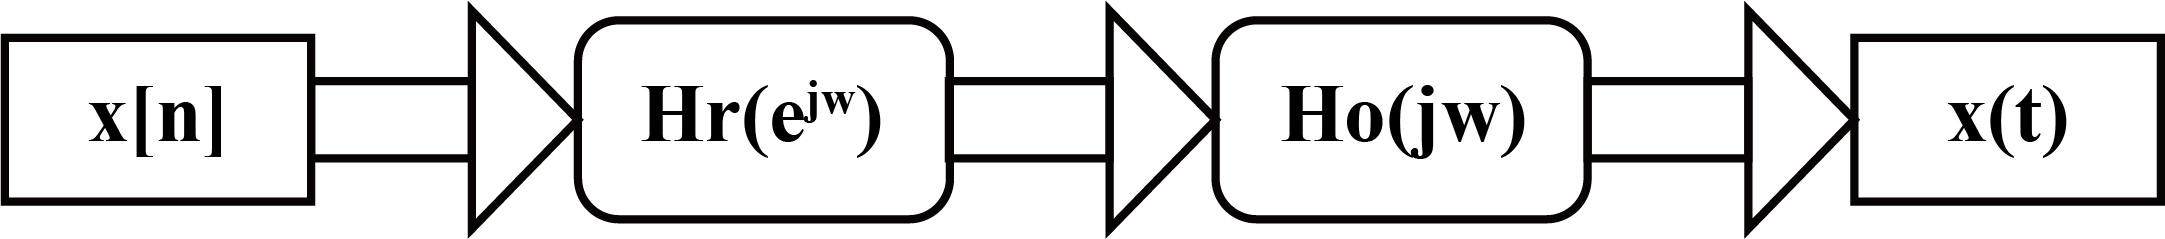
\includegraphics[width = 0.7\textwidth]{pic/sys2.png}
                \caption{离散预矫正系统}
            \end{figure}

        \subsection{离散数字滤波器$H_{r}\left(e^{j \omega}\right)$的设计}
        
            此实验中我们基于$FIR$滤波器的频率采样设计方法,设计离散系统数字滤波器$H_{r}\left(e^{j \omega}\right)$。
            
            系统的连续系统频率响应的模为(以下分析中暂时忽略1/T的增益):
            
            $$H_{r}(j \omega)=\frac{\omega T / 2}{\sin (\omega T / 2)},|\omega|<\omega_{c}$$
            
            根据采样序列与原信号的关系有:
            
            $$H_{r}\left(e^{j v}\right)=H_{r}\left(j \frac{\omega}{T}\right)=\frac{\omega / 2}{\sin (\omega / 2)}$$

            对$H_{r}\left(e^{j \omega}\right)$进行等间隔采样,得:
            
            $$H_{r}(m)=\left.H_{r}\left(e^{j v}\right)\right|_{\omega = \frac{2 \pi m}{N}}=\frac{\pi m / N}{\sin (\pi m / N)}$$
                    
            假设是对$H_{r}\left(e^{j \omega}\right)$在一个周期内采样$(2 \mathrm{M}+1)$个点,可得:
            
            $$h_{r}[n]=\frac{1}{2 M+1} \sum_{m=0}^{2 M} H_r(m) e^{j m n \frac{2 n}{2 M+1}}$$
            
            若假设采样点很多,即$2 \mathrm{M}>>1$,利用$H_r\left(e^{j \omega}\right)$的周期性,可得:
            
            $$h_{r}[n]=\frac{1}{2 M} \sum_{m=M}^{M} \frac{m \pi / 2 M}{\sin (m \pi / 2 M)} e^{j m n / M}$$
            
            当$m=O$时,$h_r[n]$化简为:
            
            $$h_{r}[n]=\frac{1}{M}\left[\frac{1}{2}+\sum_{m=1}^{M} \frac{m \pi / 2 M}{\sin (m \pi / 2 M)} \cos (m n \pi / M)\right]$$
            
            将$h_{r}[n]$进行离散信号傅立叶变换,并利用 $H\left(e^{j \omega}\right)=H\left(j \frac{\omega}{T}\right)$当关系,可得连续频率变量的滤波器频响函数如下:
            
            $$H_{r}{ }^{\prime}(j \omega)=H_{r}{ }^{\prime}\left(e^{j \omega T}\right)=\sum_{n=-\infty}^{\infty} h_r[n] e^{-j n \omega T} \approx \sum_{n=-N}^{N} h_r[n] e^{-j n \omega T}$$
            
            当N足够大时,$H_{r}{ }^{\prime}(j \omega)$可简化为:
            
            $$H_{r}^{\prime}(j \omega)=h[0]+2 \sum_{n=1}^{N} h_r[n] \cos n \omega T$$

            是非因果系统,但是根据FIR滤波器的特点,由于$h_{r}[n]$ 两边都趋向于零,只需将$h_{r}[n]$ 信号截取一段然后作适当的平移即可将系统改为因果系统,这样处理后对冲激信号的频谱幅值是无影响的,仅是在相位上有一个线性叠加。延时后得到的是一个有恒定群延时的因果滤波器。


    \section{实验/仿真验证}
            利用Matlab软件对设计出的滤波器和系统进行仿真,并且进行信号重建实验。

            仿真中输入测试信号如图3所示,其频谱$\omega _m = 5 $,采样周期T = 0.5,$\omega _s = 4 \pi > 2 \omega_m$,满足采样定理。

            图4是利用公式$H r(j \omega)= \frac{\omega T / 2}{\sin (\omega T / 2)}$画出的理想的连续时间系统的频率响应图。

            图5是利用公式$H_{r}^{\prime}(j \omega)=h[0]+2 \sum_{n=1}^{N} h_r[n] \cos n \omega T$画出的离散数字系统的频率响应图。

            比较两个图,可以看到,在$- \frac{\omega_s}{2} \sim \frac{\omega_s}{2}$范围内发现两条曲线比较吻合。

            将$H_o(j\omega)$和$H_{r}^{\prime}(j \omega)$级联(相乘),得到重建后的理想滤波器$H(j \omega)$如图6所示,可以看到在$- \frac{\omega_s}{2} \sim \frac{\omega_s}{2}$范围内滤波器的增益非常接近1,效果很好。
            
            \begin{figure}[H]
                \centering
                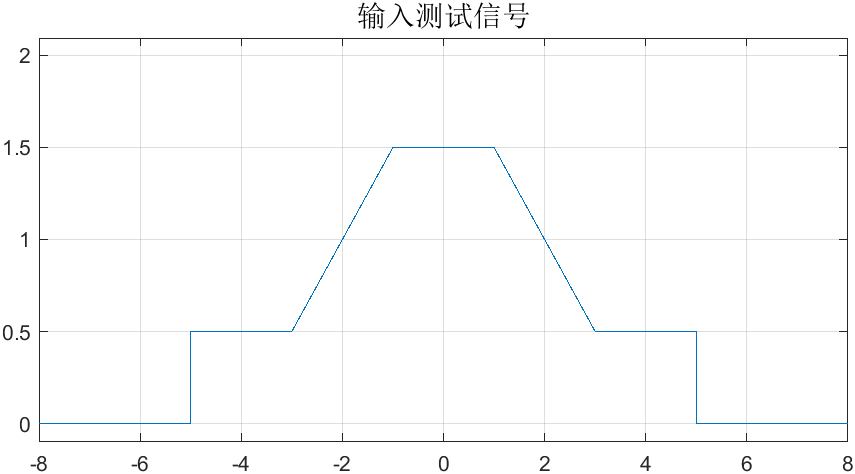
\includegraphics[width=0.6\textwidth]{pic/输入测试信号.png}
                \caption{输入测试信号}
            \end{figure}
            \begin{figure}[H]
                \centering
                
                \begin{minipage}[t]{0.48\textwidth}
                    \centering
                    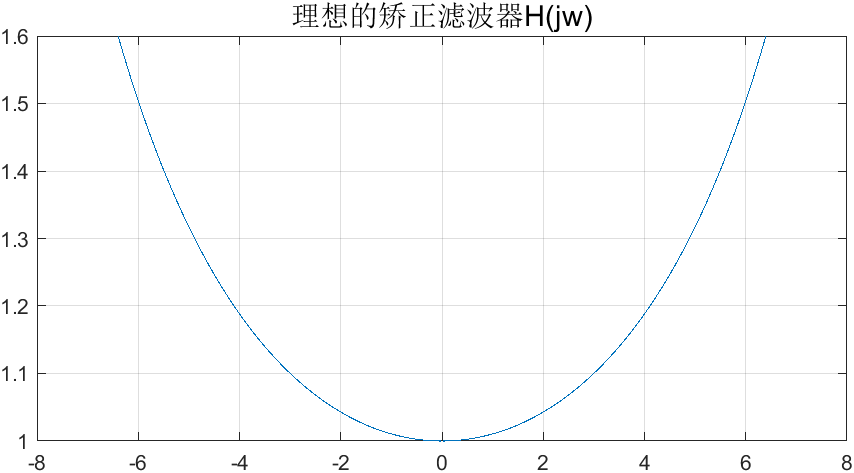
\includegraphics[width=0.9\textwidth]{pic/理想的矫正滤波器H(jw).png}
                    \caption{理想的矫正滤波器$H(jw)$}
                \end{minipage}
                \begin{minipage}[t]{0.48\textwidth}
                    \centering
                    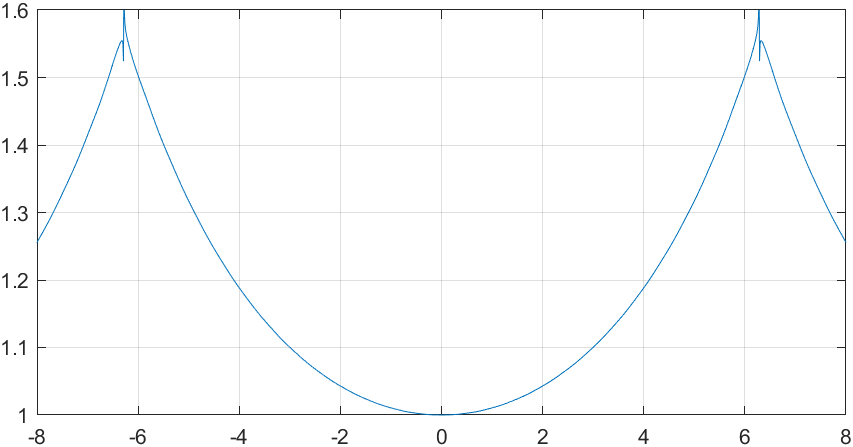
\includegraphics[width=0.9\textwidth]{pic/重建后的Hr'(jw).png}
                    \caption{重建后的$H_{r}{ }^{\prime}(j \omega)$}
                \end{minipage}

                \vspace{15pt}

                \begin{minipage}[t]{0.48\textwidth}
                    \centering
                    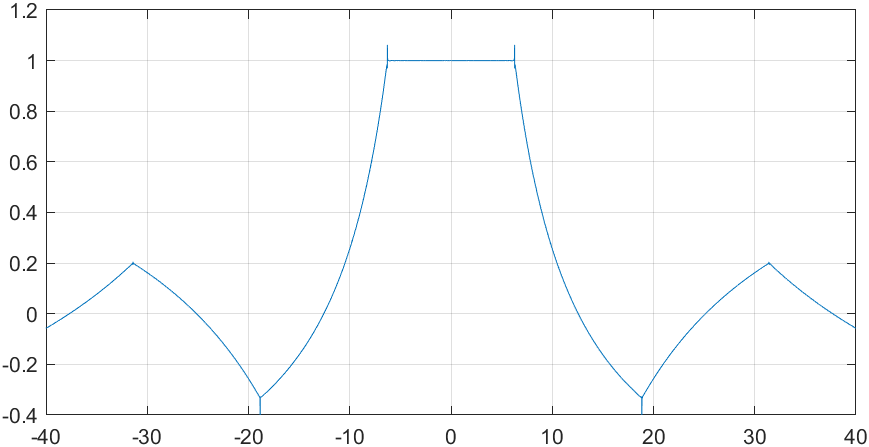
\includegraphics[width=0.9\textwidth]{pic/重建后的联合滤波.png}
                    \caption{重建后的联合滤波}
                \end{minipage}
                \begin{minipage}[t]{0.48\textwidth}
                    \centering
                    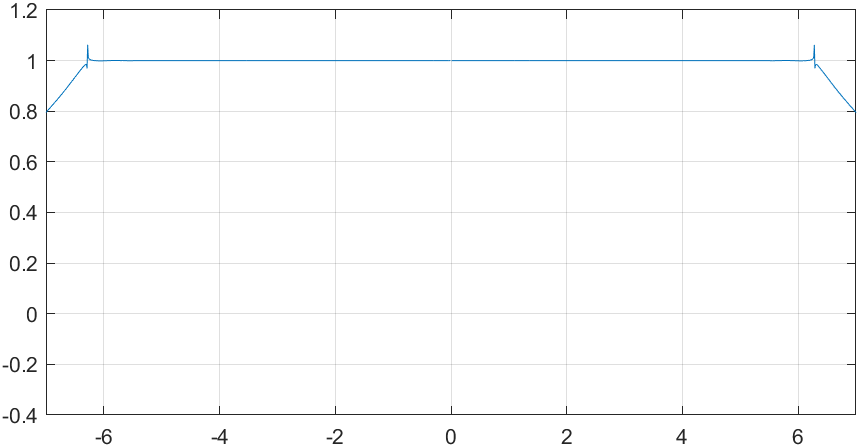
\includegraphics[width=0.9\textwidth]{pic/联合局部放大.png}
                    \caption{重建后的联合滤波局部放大}
                \end{minipage}

                \vspace{15pt}

                \begin{minipage}[t]{0.48\textwidth}
                    \centering
                    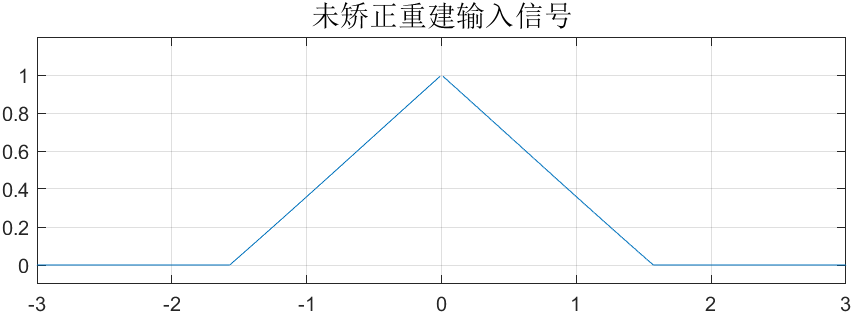
\includegraphics[width=0.9\textwidth]{pic/未矫正重建输入信号.png}
                    \caption{未矫正重建输入信号}
                \end{minipage}
                \begin{minipage}[t]{0.48\textwidth}
                    \centering
                    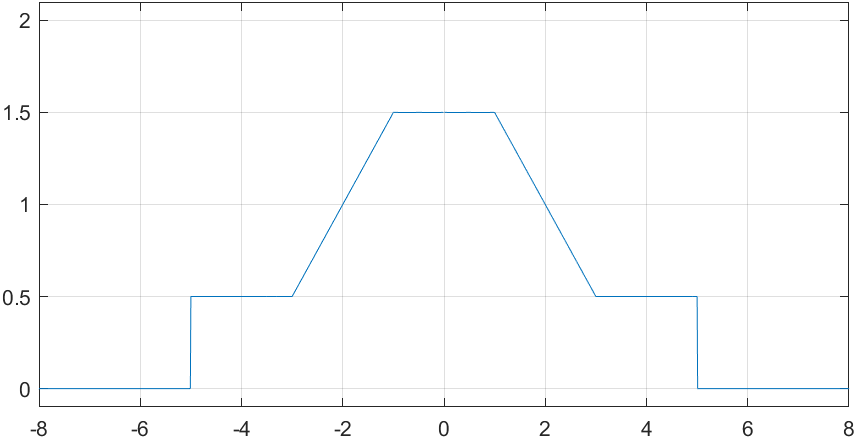
\includegraphics[width=0.9\textwidth]{pic/矫正后重建输入信号.png}
                    \caption{矫正后重建输入信号}
                \end{minipage}
            \end{figure}

            \begin{figure}[H]
                \centering
                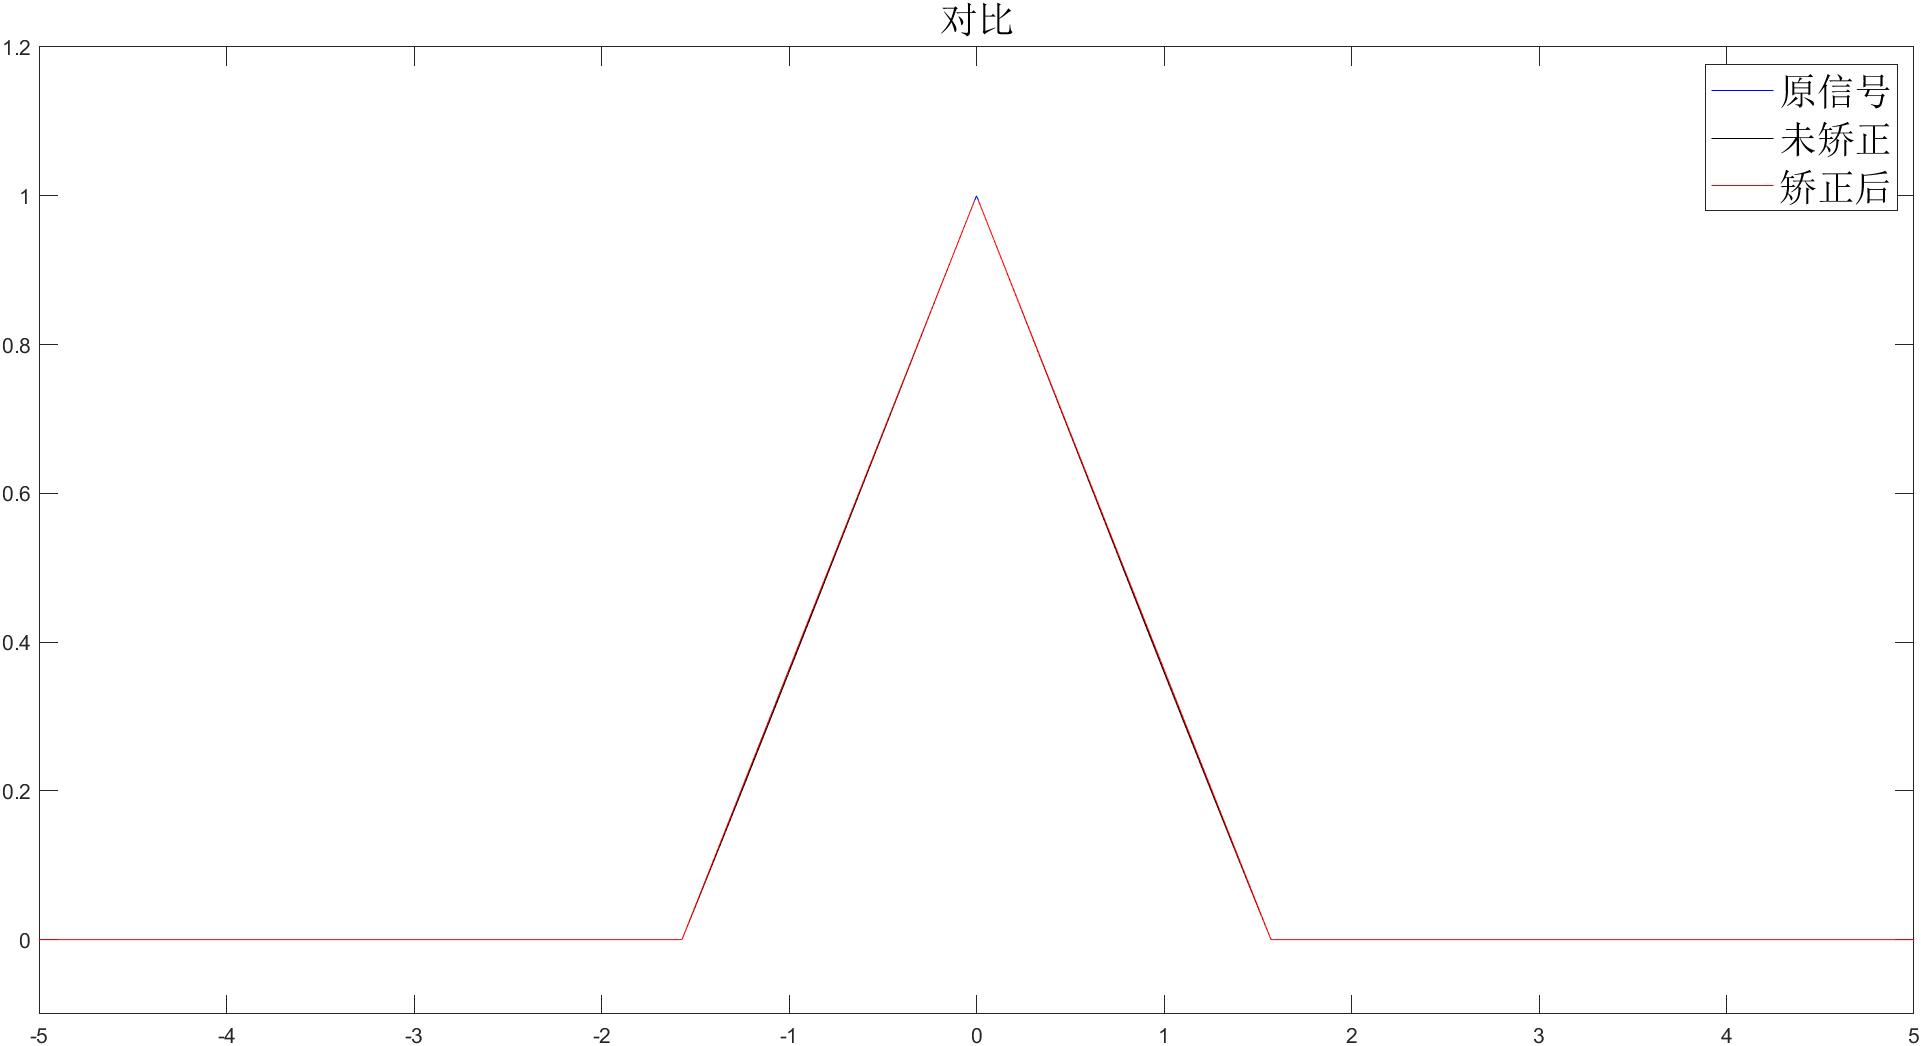
\includegraphics[width=0.7\textwidth]{pic/对比.png}
                \caption{对比图}
            \end{figure}
            \begin{figure}[H]
                \centering
                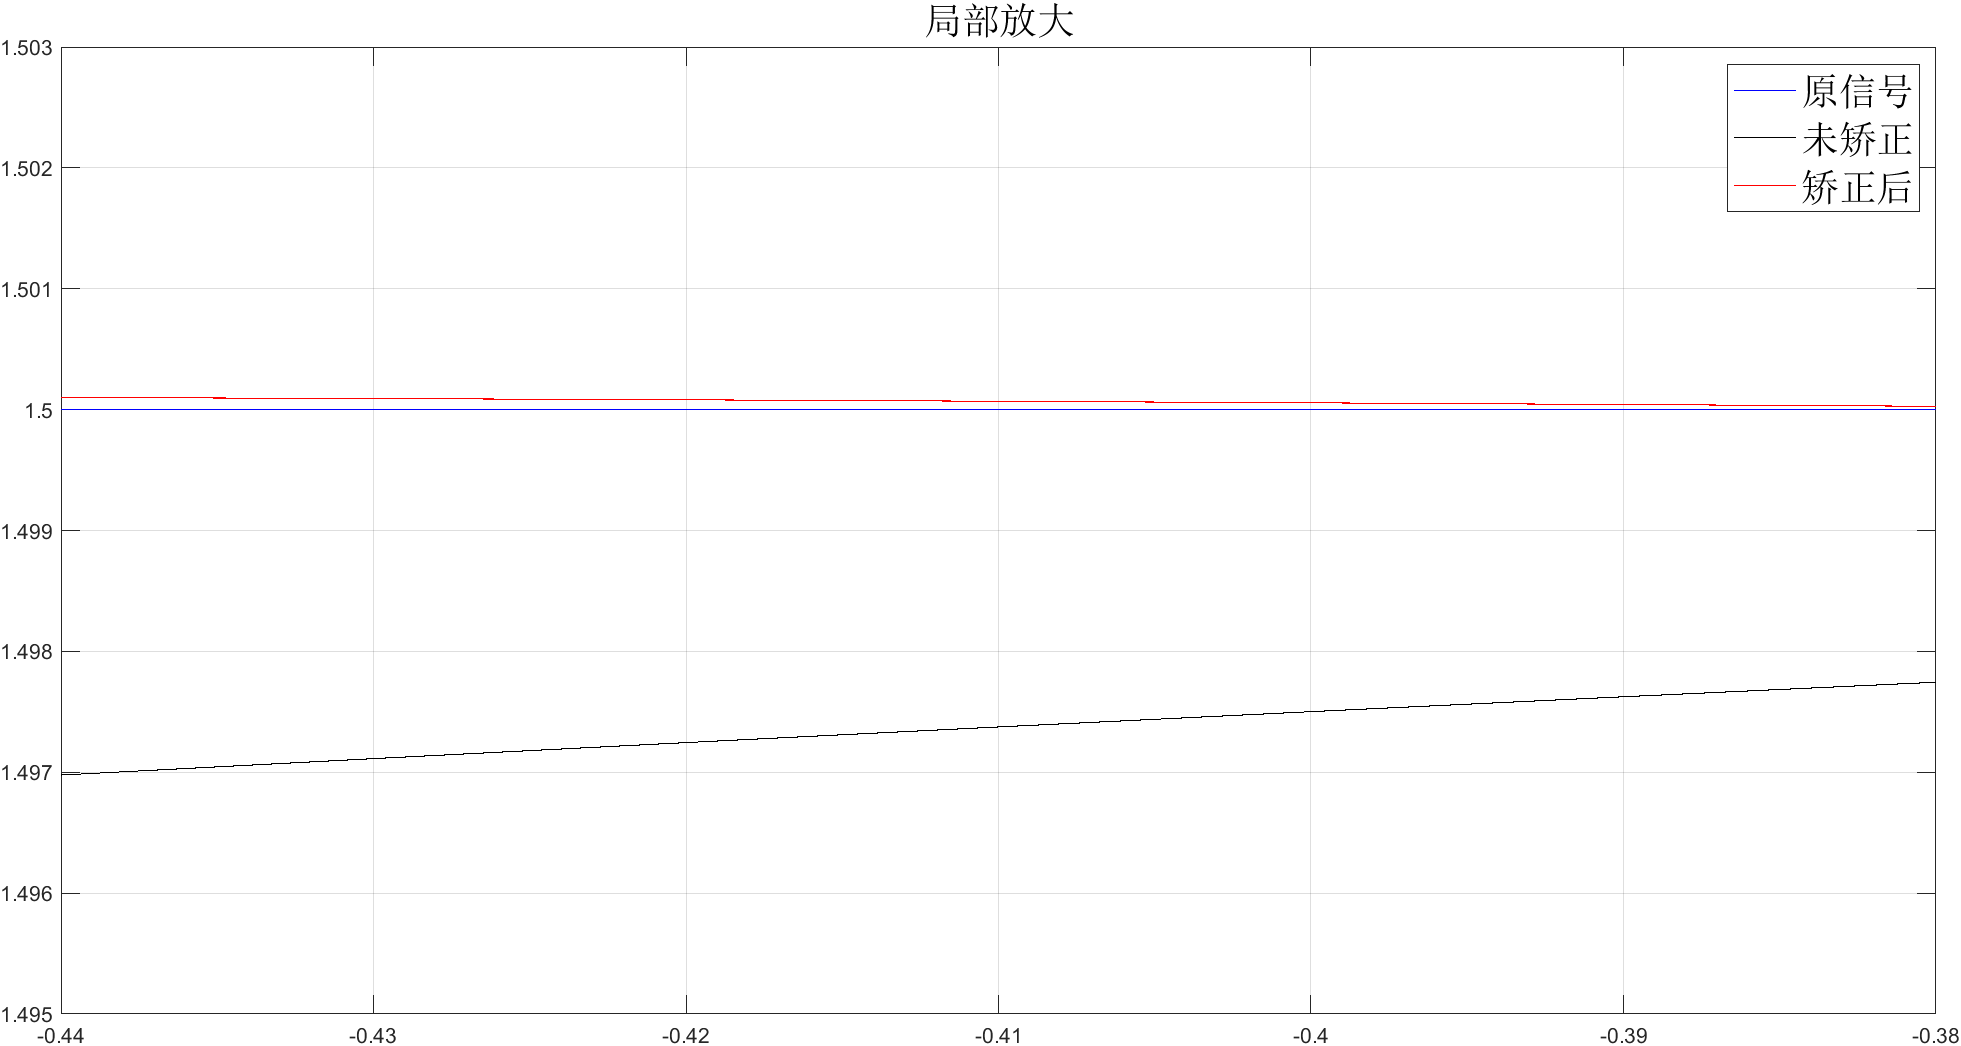
\includegraphics[width=0.7\textwidth]{pic/局部放大.png}
                \caption{对比图-局部放大}
            \end{figure}

            而对比直接用零阶保持系统$H_o(jw)$恢复的信号(图8:未校正的重建输入信号)和通过将$H_o(j\omega)$和$H_{r}^{\prime}(j \omega)$级联(相乘),得到重建后的理想滤波器恢复的信号(图9:矫正后重建输入信号),如图10,可以看到矫正后重建输入信号和输入信号非常吻合,从局部放大图(图11)来看差距也非常小。说明设计成功。
    \section{结论和心得}
        从仿真结果可以看出,设计的基于FIR滤波器的预矫正系统,很好地重建了信号,解决了数模转换中频谱失真问题。

        通过本次大作业,我对FIR滤波器的认识更加深入了。同时对Matlab软件的使用也更加熟练。

    \section{实验设计代码}

    \lstinputlisting[
        language       =   Matlab,
        title     =   {主程序}
    ]{src/test.m}

    \lstinputlisting[
        language       =   Matlab,
        title     =   {零阶保持系统$H_o(jw)$}
    ]{src/Hw.m}

    \lstinputlisting[
        language       =   Matlab,
        title     =   {理想的矫正滤波器$H_r(jw)$}
    ]{src/Hw2.m}

    \lstinputlisting[
        language       =   Matlab,
        title     =   {$h_r[n]$}
    ]{src/hrn.m}

    \lstinputlisting[
        language       =   Matlab,
        title     =   {重建后的$H_{r}^{\prime}(j \omega)$}
    ]{src/Hrw.m}
    
\end{document}